\documentclass[t,aspectratio=169]{beamer}
\usetheme[progressbar=frametitle]{metropolis}
\usefonttheme{professionalfonts}
\usepackage{appendixnumberbeamer}

\usepackage{booktabs}
\usepackage[scale=2]{ccicons}

\usepackage{graphics,graphicx,amssymb,amsmath,pgf,comment,hyperref}
%\usepackage[xcolor=pst]{pstricks}
\usepackage{array}
\usepackage{pgfshade}
\usepackage[round]{natbib}
\usepackage[absolute,overlay]{textpos}
\usepackage{pifont}
\usepackage{dcolumn}
\usepackage{textpos}
\usepackage{color}					
\usepackage{xcolor,colortbl}
\usepackage{tikz}
\usepackage{bbm}
\usepackage{curves}
\usepackage{mathtools}
\usepackage{times}
\usepackage{verbatim}
\usetikzlibrary{snakes,arrows,shapes,positioning}
\def\augie{\fontencoding{T1}\fontfamily{augie}\selectfont}

\usepackage{pgfplots}
\usepgfplotslibrary{dateplot}
\usepackage{bm}

\usepackage{xspace}
\newcommand{\themename}{\textbf{\textsc{metropolis}}\xspace}

\definecolor{beamcol}{RGB}{5,48,97}
\definecolor{beamcol2}{RGB}{33,102,172}
\usecolortheme[named=beamcol]{structure}

\setbeamertemplate{caption}{\raggedright\insertcaption\par}
\usetikzlibrary{calc,decorations.pathmorphing,patterns}
\pgfdeclaredecoration{penciline}{initial}{
    \state{initial}[width=+\pgfdecoratedinputsegmentremainingdistance,
    auto corner on length=1mm,]{
        \pgfpathcurveto%
        {% From
            \pgfqpoint{\pgfdecoratedinputsegmentremainingdistance}
                      {\pgfdecorationsegmentamplitude}
        }
        {%  Control 1
        \pgfmathrand
        \pgfpointadd{\pgfqpoint{\pgfdecoratedinputsegmentremainingdistance}{0pt}}
                    {\pgfqpoint{-\pgfdecorationsegmentaspect
                     \pgfdecoratedinputsegmentremainingdistance}%
                               {\pgfmathresult\pgfdecorationsegmentamplitude}
                    }
        }
        {%TO
        \pgfpointadd{\pgfpointdecoratedinputsegmentlast}{\pgfpoint{1pt}{1pt}}
        }
    }
    \state{final}{}
}


\title{Owning the Agent: Hospital Influence on Physician Behaviors}
\date{}
\author{Haizhen Lin \& \textbf{Ian McCarthy} \& Michael Richards}
\institute{November 15, 2019}

\begin{document}
\maketitle

\section{Motivation}

\begin{frame}[t]{Hospital in Physician Agency Problem}
\bigskip
    \begin{tikzpicture}
    % draw horizontal line
    \draw[thick, -] (1cm,0) -- (10cm,0);

    % draw node
    \draw[ultra thick] (1,0) node[left=3pt,thick] {Physician};
    \draw[ultra thick] (10,0) node[right=3pt,thick] {Patient};

    \only<2-3>{
        % draw and label vertical lines
        \draw[thick, -] (4 cm,7pt) -- (4 cm,-7pt);
        \draw[thick, -] (7 cm,7pt) -- (7 cm,-7pt);
        \draw[thick] (7, -1) node(Pat)[above=1pt] {$y_{1}$};
        \draw[thick] (4, -1) node(Phy)[above=1pt] {$y_{2}$};
    }

    \only<3>{
        \draw[ultra thick] (7,-3) node(ur)[above=3pt,thick] {Hospital};
        \draw [beamcol, thick, ->] (ur) [in = 270] to [out = 60]  (Pat);
        \draw [beamcol, thick, ->] (ur) [in = 270] to [out = 120]  (Phy);
    }

    \only<4-6>{
        \draw[thick, -] (5 cm,6pt) -- (5 cm,-6pt);
        \draw[thick] (5, -1) node(Pat)[above=1pt] {$y^{*}$};
    }

    \only<5-6>{
        \draw[ultra thick] (0,-0.4) node[thick] {\& Hospital};
    }

    \only<6>{
        \draw[thick, ->] (4.8, -1) -- (3.2,-1);
        \draw[thick, -] (3 cm,6pt) -- (3 cm,-6pt);
        \draw[thick] (3, -1) node(Phy)[above=1pt] {$y^{*}_{h}$};
    }
    \end{tikzpicture}

\end{frame}

\tikzstyle{every picture}+=[remember picture]
\everymath{\displaystyle}
\begin{frame}{Changing Physician Relationships}
    \begin{figure}
        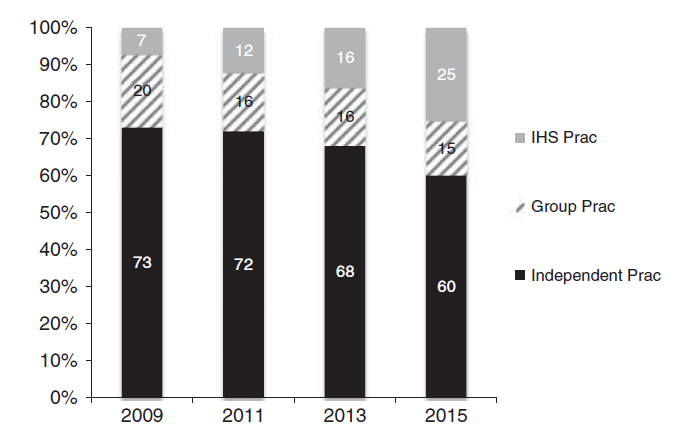
\includegraphics[height=2.4in,keepaspectratio]{Richardsetal.png}
        \caption{Richards \textit{et al.}, Medical Care, 2016}
    \end{figure}
\end{frame}

\begin{frame}{In context}
    \begin{itemize}
        \item Physician agency (Clemens \& Gottlieb 2014, AER; Afendulis \& Kessler 2007, AER; Gruber \& Owings 1996, RAND; Iizuka 2012, AER)
        \item Supply-side variation (Finkelstein \textit{et al.} 2016, QJE; Molitor 2018, AEJ: Policy)
        \item Vertical integration (Cuellar \& Gertler 2006, JHE; Ciliberto \& Dranove 2006, JHE; Baker \textit{et al.} 2016, JHE; Koch \textit{et al.} 2017, JHE)
    \end{itemize}
\end{frame}

\begin{frame}{Outline}
    \begin{enumerate}
        \item Estimation strategy
        \item Initial Results
        \item Event Study, DDD, Quantile, IV
        \item Treatment intensity vs reallocation
        \item Other Outcomes
    \end{enumerate}
\end{frame}

\section{Estimation Strategy}
\begin{frame}{Estimation Strategy}
    \tikzstyle{na} = [baseline=-.5ex]
    \only<1->{
        Observed care at time $t$ is
        \begin{equation*}
            y_{ijk} =
            \tikz[baseline]{
                \node[fill=blue!20,anchor=base] (t1)
                {$ \alpha_{i} + x_{i}\beta $};
            } +
            \tikz[baseline]{
                \node[fill=red!20, ellipse, anchor=base] (t2)
                {$\Gamma_{jk}$};
            } + \epsilon_{ijk}
        \end{equation*}
        \begin{itemize}[<+-| alert@+>]
            \item[]<2-> Patient Preferences
                \tikz[na] \node[coordinate] (n1) {};
            \item[]<3-> Physician and hospital characteristics
                \tikz[na] \node[coordinate] (n2) {};
        \end{itemize}

        \begin{tikzpicture}[overlay]
            \path[->]<2-> (n1) edge [bend right] (t1);
            \path[->]<3-> (n2) edge [out=0, in=-90] (t2);
        \end{tikzpicture}
    }
\end{frame}

\begin{frame}{Physician-hospital ``match value''}
    \tikzstyle{na} = [baseline=-.5ex]

    \only<1>{
        Two-step approach:
        \begin{enumerate}
            \item Estimate patient-level regression (separately by year): $$y_{ijk} = \alpha_{i} + x_{i}\beta + \Gamma_{jk} + \epsilon_{ijk}$$
            \item Estimate physician/hospital-level regression in panel: $$\hat{\Gamma}_{jkt} = \gamma_{j} + \gamma_{k} + \tau_{t} + z_{jkt}\delta + \eta_{jkt}$$
        \end{enumerate}
    }
    \only<2-6>{
        \begin{equation*}
            y_{ijk} = \alpha_{i} + x_{i}\beta + \underbrace{
            \tikz[baseline]{
                \node[fill=blue!20,anchor=base] (t1)
                {$\Gamma_{jk}^{t}$};
            }}_{
            \tikz[baseline]{
                \node[fill=green!20,anchor=base] (t2)
                {$\Gamma_{j}$};
            } +
            \tikz[baseline]{
                \node[fill=red!20,anchor=base] (t3)
                {$\Gamma_{k}$};
            } +
            \tikz[baseline]{
                \node[fill=orange!20,ellipse,anchor=base] (t4)
                {$z_{jkt}\delta$};
            }} +
            \epsilon_{ijk}
        \end{equation*}
        \begin{itemize}[<+-| alert@+>]
            \item[]<3-> Physician, hospital, and match effect (jointly)
                \tikz[na] \node[coordinate] (n1) {};
            \item[]<4-> Physician effect
                \tikz[na] \node[coordinate] (n2) {};
            \item[]<5-> Hospital effect
                \tikz[na] \node[coordinate] (n3) {};
            \item[]<6-> Physician-hospital integration
                \tikz[na] \node[coordinate] (n4) {};
        \end{itemize}

        \begin{tikzpicture}[overlay]
            \path[->]<3-> (n1) edge [out=0, in=-90] (t1);
            \path[->]<4-> (n2) edge [out=10, in=-70] (t2);
            \path[->]<5-> (n3) edge [out=5, in=-80] (t3);
            \path[->]<6-> (n4) edge [out=0, in=-90] (t4);
        \end{tikzpicture}
    }
    \only<7>{
        \begin{itemize}
            \item Draws from ``match values'' in labor literature (Abowd \textit{et al.}, 2002; Card \textit{et al.}, 2013, QJE )
            \item Exploits variation across inpatient stays and splits the separation of match value into two steps
            \item Identifies effects on match value from within-physician variation across hospitals
        \end{itemize}
    }
\end{frame}


\section{Data}
\begin{frame}{Data Sources}
    \begin{itemize}
        \item<1-> CMS: 100\% inpatient and institutional outpatient Medicare claims data (2008-2015)
        \item<1-> SK\&A: Hospital ownership of physician practices and practice characteristics
        \item<2-> AHA, HCRIS, POS: Hospital characteristics
        \item<2-> Annual IPPS Impact Files: Hospital cost-to-charge ratios (CCR)
        \item<2-> ACS: County-level demographics, education, income, and employment
    \end{itemize}
\end{frame}

\begin{frame}{Sample Construction}
    \begin{itemize}
        \item<1-> Planned inpatient stays (elective admissions initiated by a physician, clinic, or HMO referral) and outpatient procedures with observed NPI for the operating physician
        \item<2-> Drop physicians operating in hospitals more than 120 miles from primary office or outside of contiguous U.S.
        \item<2-> Drop physicians with NPIs not matched in the SK\&A data
        \item<2-> Drop lowest/highest 1\% of charges and patients $<$ 65 years old
    \end{itemize}
  \uncover<3->{ $\longrightarrow$ 518,398 unique observations at the physician/hospital/year \\
   $\longrightarrow$ 7.5mm inpatient stays (47\% of total) and 24mm outpatient procedures}
\end{frame}

\section{Preliminary Evidence}
\begin{frame}{Total Spending by Integration Status}
    \only<1>{
        Estimate and plot residual from:
        \begin{equation*}
            y_{jkt} = \beta x_{jt} + \delta z_{kt} + \lambda_{k} + \lambda_{j} + \lambda_{t} + \varepsilon_{jkt}
        \end{equation*}
    }
    \only<2>{
        \begin{figure}
            \centering
            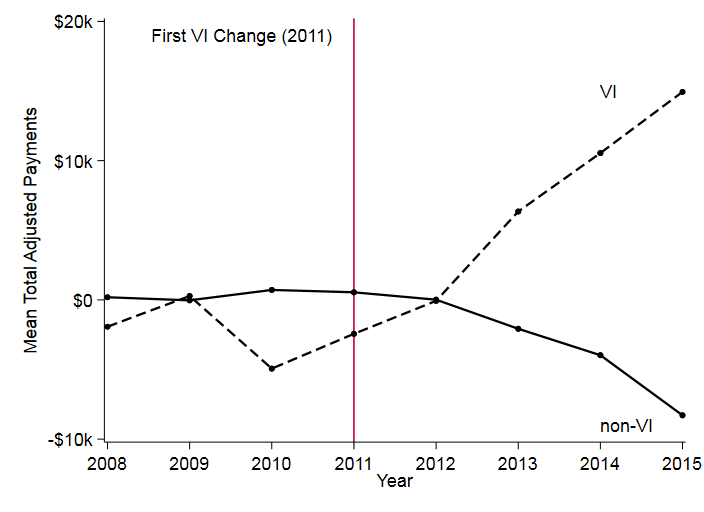
\includegraphics[height=2.5in,width=5in,keepaspectratio]{Summary_Pay3}
        \end{figure}
    }
\end{frame}


\section{Vertical Integration and Match Values}
\begin{frame}{Estimated Effects of Vertical Integration}
    \only<1>{
    Two-step estimation strategy:
    \begin{enumerate}
        \item Estimate $y_{ijk} = \alpha_{i} + x_{i}\beta + \Gamma_{jk} + \epsilon_{ijk}$ at patient level (separately by year)
        \item Estimate $\hat{\Gamma}_{jkt} = \gamma_{j} + \gamma_{k} + \tau_{t} + z_{jkt}\delta + \eta_{jkt}$ with physician-hospital panel
    \end{enumerate}
    }
    \only<2->{
    \begin{equation*}
        \hat{\Gamma}_{jkt} = \gamma_{j} + \gamma_{k} + \tau_{t} + z_{jkt}\delta + \eta_{jkt},
    \end{equation*}
    }
    \only<3->{
        \begin{table}[htb!]
        \centering
        \centerline{
        \begin{tabular}{l|rr}
            Outcome & Estimate & St. Error \\
            \hline\hline \onslide<4->{\vspace{-.1in}\\
            Total Medicare Payments & 76.176** & (30.911)  \onslide<5->{\\
            Total Hospital Costs & 133.063***  & (42.099) \onslide<6->{\\
            Total Procedures   &   0.014***  &  (0.004) }}}\\
            \hline
            \multicolumn{3}{l}{\footnotesize * p-value $<$0.1, ** p-value $<$0.05, *** p-value $<$0.01}
        \end{tabular}}
        \end{table}
    }
\end{frame}


\begin{frame}{Threats to Identification and Interpretation}
    Two-way fixed effects estimator with time varying treatment...
    \only<2>{
        \metroset{block=fill}
        \begin{block}{Potential Problems}
            \begin{enumerate}
                \item \textbf{Endogeneity:} Vertical integration due to time-varying unobservables \& outcomes (standard DD/2WFE concern)
                \item \textbf{Interpretation:} Weighted average of all 2$\times$2 DD estimates, with some potentially negative weights
            \end{enumerate}
        \end{block}
    }
\end{frame}


\section{Event Studies}
\begin{frame}{Total Medicare Payments}
    \begin{figure}
        \centering
        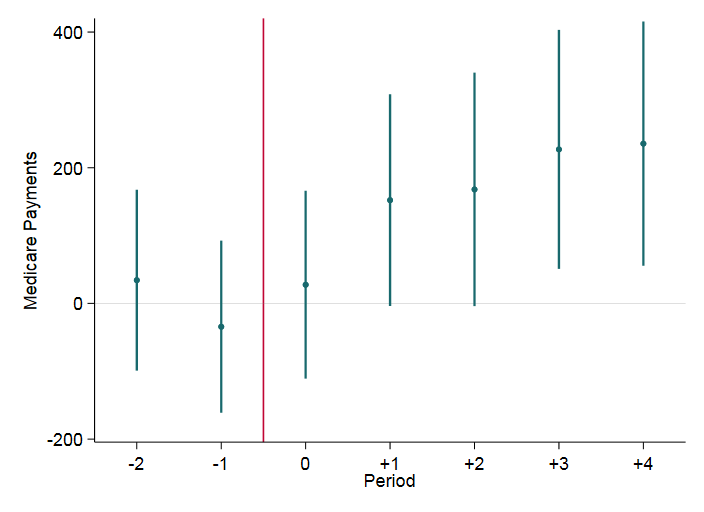
\includegraphics[height=2.5in,width=5in,keepaspectratio]{EventPay_All_2011}
    \end{figure}
\end{frame}

\begin{frame}{Total Hospital (IP \& OP) Costs}
    \begin{figure}
        \centering
        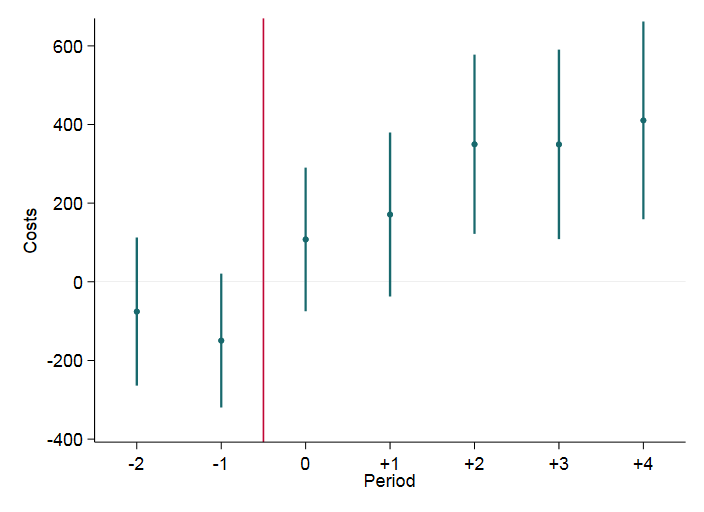
\includegraphics[height=2.5in,width=5in,keepaspectratio]{EventCharge_All_2011}
    \end{figure}
\end{frame}

\begin{frame}{Takeaways}
    \begin{itemize}
        \item Increase in payments and costs
        \item Evidence consistent with common trends assumption for total payments and costs
        \item Concerns about limited pre-period data
    \end{itemize}
\end{frame}

\section{Triple Difference}
\begin{frame}{Triple Difference}
\only<1->{
    \begin{equation*}
            \hat{\Gamma}_{jkt} = \gamma_{j} + \gamma_{k} + \tau_{t} + \underbrace{
            \tikz[baseline]{
                \node[anchor=base] (t1) {$z_{jkt} \delta $};
            }}_{
            \tikz[baseline]{
                \node[anchor=base] (t2) {$1\left( VI_{j} \right) \delta_{1} $};
            } +
            \tikz[baseline]{
                \node[anchor=base] (t3) {$1\left( VI_{j,k} \right) \delta_{2}$};
            } +
            \tikz[baseline]{
                \node[anchor=base] (t4) {$z_{jkt} \mu $};
            }} +
            \eta_{jkt}
    \end{equation*}
}
\only<2->{
    \begin{table}[htb!]
    \centering
    \centerline{
    \begin{tabular}{l|rr|rr}
                & \multicolumn{2}{l}{Integration, $(j, k)$} & \multicolumn{2}{|l}{Integration, $j$} \\
        Outcome & Estimate & St. Error & Estimate & St. Error \\
        \hline\hline \onslide<3->{\vspace{-.1in}\\
        Total Medicare Payments & 185.041** & (79.809) & -18.611 & (103.835) \onslide<4->{\\
        Total Hospital Costs & 32.362  & (109.502) & 309.161*** & (147.166) \onslide<5->{\\
        Total Procedures   &   0.023**  &  (0.010) & -0.014 & (0.011) }}}\\
        \hline
        \multicolumn{5}{l}{\footnotesize * p-value $<$0.1, ** p-value $<$0.05, *** p-value $<$0.01}
    \end{tabular}}
    \end{table}
}
\end{frame}

\section{Heterogeneous Effects}
\begin{frame}{Unconditional Quantile Results: Payments}
    \begin{figure}
        \centering
        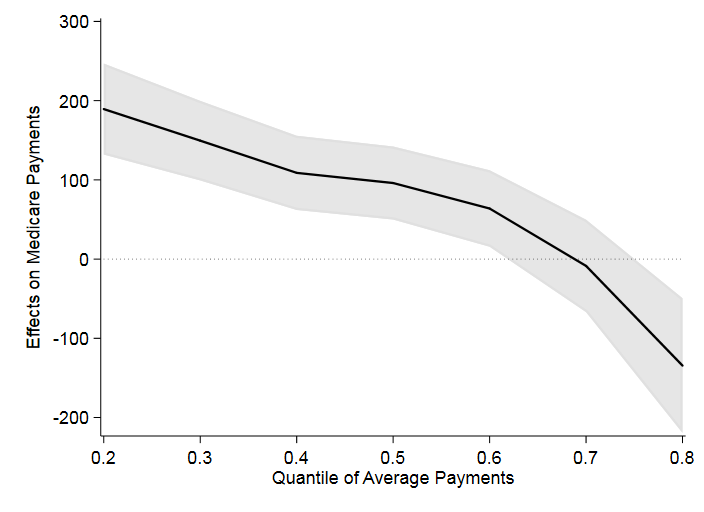
\includegraphics[height=2.5in,width=5in,keepaspectratio]{QReg_Payment}
    \end{figure}
\end{frame}

\begin{frame}{Unconditional Quantile Results: Hospital Costs}
    \begin{figure}
        \centering
        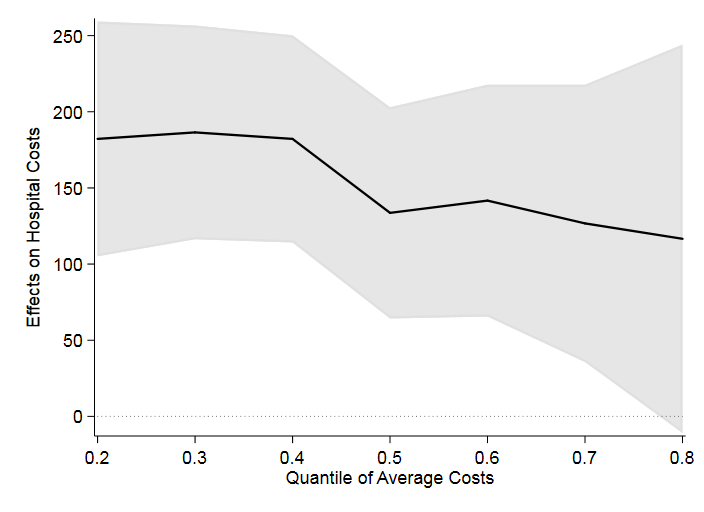
\includegraphics[height=2.5in,width=5in,keepaspectratio]{QReg_Charge}
    \end{figure}
\end{frame}

\begin{frame}{Unconditional Quantile Results: Procedures}
    \begin{figure}
        \centering
        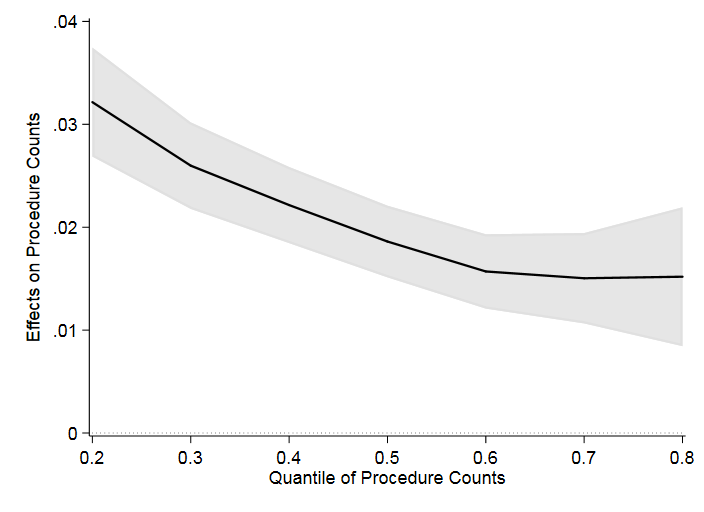
\includegraphics[height=2.5in,width=5in,keepaspectratio]{QReg_Procs}
    \end{figure}
\end{frame}

\section{Treatment Intensity vs Reallocation}

\begin{frame}{Want to isolate treatment intensity effect}
    \begin{enumerate}
        \item Focus on patients with no change in physician/hospital pairs over time
        \item Examine outcomes within an inpatient stay
    \end{enumerate}
\end{frame}

\begin{frame}{Aggregate Outcomes without Reallocation}
    \vspace{0.75in}
    \begin{table}[htb!]
    \centering
    \centerline{
    \begin{tabular}{l|rr}
        Outcome & Estimate & St. Error \\
        \hline\hline \onslide<2->{\vspace{-.1in}\\
        Total Medicare Payments & 64.134** & (30.858)  \onslide<3->{\\
        Total Hospital Costs & 122.894***  & (42.130) \onslide<4->{\\
        Total Procedures & 0.013** & (0.004) }}}\\
        \hline
        \multicolumn{3}{l}{\footnotesize * p-value $<$0.1, ** p-value $<$0.05, *** p-value $<$0.01}
    \end{tabular}}
    \end{table}
\end{frame}

\begin{frame}{Effects on Components of Inpatient Stay}
    \vspace{0.5in}
    \begin{table}[htb!]
    \centering
    \centerline{
    \begin{tabular}{l|rr}
        Outcome & Estimate & St. Error \\
        \hline\hline
        Charges for: & & \\
        \hspace{.1in} Total Inpatient & 180.997*** & (49.771) \\
        \hspace{.1in} Medical Supplies & 40.564 & (30.024) \\
        \hspace{.1in} Operating Room & -11.029 & (22.928) \\
        \hspace{.1in} Anesthesia & 5.278 & (4.999) \\
        \hspace{.1in} Labs & 9.286 & (8.826) \\
        \hspace{.1in} Radiology & -5.943 & (6.058) \\
        \hspace{.1in} MRI & -0.514 & (1.359) \\
        \hline
        \multicolumn{3}{l}{\footnotesize * p-value $<$0.1, ** p-value $<$0.05, *** p-value $<$0.01}
    \end{tabular}}
    \end{table}
\end{frame}

\begin{frame}{Effects on Components of Inpatient Stay}
    \vspace{0.5in}
    \begin{table}[htb!]
    \centering
    \centerline{
    \begin{tabular}{l|rr}
        Outcome & Estimate & St. Error \\
        \hline\hline
        Counts of: & & \\
        \hspace{.1in} ICU Days  & 0.021  & (0.013) \\
        \hspace{.1in} Procedures  & 0.030*** & (0.009) \\
        \hline
        \multicolumn{3}{l}{\footnotesize * p-value $<$0.1, ** p-value $<$0.05, *** p-value $<$0.01}
    \end{tabular}}
    \end{table}
\end{frame}

\begin{frame}{Other Effects}
    Other ways integration posited to affect physician behavior:
    \begin{itemize}
        \item More procedures overall (not per patient)
        \item Reallocating procedures from other hospitals
        \item Reallocating procedures across inpatient and outpatient settings
        \item Changing patient profile
    \end{itemize}
\end{frame}

\section{Main Takeaways}
\begin{frame}{Summary of Results}
    \only<1>{
        \metroset{block=fill}
        \begin{block}{Sensitivity}
           \begin{itemize}
                \item Event study, triple difference, unconditional quantile, IV
                \item Effects not driven by reallocation
                \item No improvement in quality (mortality)
                \item No effects on payments or DRG weights per inpatient stay (falsification test)
            \end{itemize}
        \end{block}
    }

    \only<2>{
        \metroset{block=fill}
        \begin{block}{Overall Results}
            \begin{itemize}
                \item Increase in Medicare payments (\$75-\$200) and hospital costs (\$130-\$350)
                \item Extrapolates to between \$55mm and \$146mm in additional Medicare payments per year
                \item 4-10\% of within-physician variation across hospitals explained by vertical integration
            \end{itemize}
        \end{block}        
    }
\end{frame}

\section*{Thank You}


\end{document}






